% INSTRUCTIONS:
% To compile this file, run "latex HW_example";  you need to do it TWICE
%    to get the cross-references (to equations, etc) to show correctly.
% Figures can be included as shown below.  If you don't have a figure,
%    comment out those lines using % signs at the beginning of each line,
%    or else just keep hitting RETURN when LaTeX gives an error message
%    saying that it can't find the figure file.
% Run "dvips HW_example.dvi" to make a Postscript file HW_example.ps,
%    and then "ps2pdf HW_example.ps" to make a PDF file HW_example.pdf.

\documentclass[12pt]{article}
\usepackage{graphicx,indentfirst}

\pagestyle{plain}
\baselineskip 18pt
\textwidth 6.5in
\textheight 7.8in
\oddsidemargin 0.1in
\evensidemargin 0.1in
\topmargin 0.3in

\newcommand{\be}{\begin{equation}}
\newcommand{\ee}{\end{equation}}
\newcommand{\reff}[1]{(\ref{#1})}


\begin{document}

\title{Computational Physics \\ Homework 3}
\author{Yi-Hsuan Hsu}
\date{10/03/2014}
\maketitle

\section{Problem 1 to 4}
\begin{equation}
	x_{n+1}=f(x)=a\times x_{n}(1-x_{n})\\
\end{equation}
Plot one-dimension map of $x_{n}]$, show the convergence behavior of $a$ in interval $[0,1]$ , $[1,3]$, $[3,3.449]$. Give analytical derivation of convergence rule in each interval.

\subsection{Theory}
Prove the global attravting stable fixed point $X*$ in each interval.

Assume that the series converges to a fixed point $x^*$, rewrite equation (1)
\begin{eqnarray}
n\rightarrow inf, x_{n+1}=x^*=f(x_{n})=ax_{n}(1-x_{n})\\
=ax^*(1-x^*)\\
x^*=1-\frac{1}{a}, or x^*=0
\end{eqnarray}
\subsubsection{ a = [0,1] , X* = 0}

When $n\rightarrow\infty$, Taylor expansion of  equation (1) $X^{*}$ in first order 
\begin{eqnarray}
	&x^*+\epsilon_{n+1}=x_{n+1}=f(x^*+\epsilon_{n})=f(x^*)+f'(x^*)*\epsilon_{n}+O(\epsilon^2)\\
	&\epsilon_{n+1}=f'(x^*)\epsilon_{n}=\lambda\epsilon_{n}
\end{eqnarray}
Where $X^{*}$ is assuming convergent to 0, $\epsilon$ is little displacement in every iteration. To show the stability of attracting point. If the $multiplier |\lambda|<1$, then $\epsilon$ would converge to 0.
\begin{equation}
	0<|\lambda|=a<1
\end{equation}
Therefore, when $0\leq a <1$, the iteration converged stably to $X*=0$.

When $a=1$, we expand Taylor series in second order, that is
\begin{eqnarray}
	x^*+\epsilon_{n+1}=f(x^*)+f'(x^*)*\epsilon_{n}+f'(x^*)\\
	\epsilon_{n+1}=\epsilon_{n}(1-\epsilon_{n})
\end{eqnarray}
Since $\epsilon$ is a small displacement, RHS alway smaller the displacement. Therefore, we may conclude that $a=1$ converge to global stable fixed point $x^*=0$.

\subsubsection{ a = [1,3] , X* = 1-1/a}
The multiplier $\lambda$
\begin{eqnarray}
	|\lambda|=|f'(x^*)|=|a(1-2(1-\frac{1}{a}))|<1\\
	1<a<3
\end{eqnarray}

\subsubsection{ a = [3.0,3.448489.....] }
In this section, the problem is nothing solving quartic equation 
\begin{equation}
	x_{n+1}g(x_{n})=f(f(x_{n}))=af(x_{n})(1-f(x_{n}))
\end{equation}
when $n\rightarrow\infty$ expand the equation and take the long division of $x$ and $x-1+\frac{1}{a}$ we can find out that
\begin{equation}
	x^*=\frac{1+a}{2a}\pm\frac{\sqrt{a^2+2a-3}}{2a^2}
\end{equation}
plug the result into multiplier, and by chain rule
\begin{equation}
	\lambda=|g(x)|=|f'(x_1)f'(x_2)|=|4+2a-a^2|<1
\end{equation}
solve a, we have$3<a<1+\sqrt6\sim3.448498....$, prove series is stable in 2-circle.
\subsubsection{find bifurcaiton point experimentally}
See Table 1.
\begin{table}[h]
	\begin{center}
		\begin{tabular}{c|c}
			\hline
			period & bifurcation point a\\ 
			\hline
			2 & $3.000$
			2 & $3.449$ \\
			4 & $3.544$\\
			8 & $3.564$\\
			16& $3.568$\\
			\hline
		\end{tabular}
	\end{center}
	\caption{Logistic output after 10000 iteration, step-in algorithm}
\end{table}

\subsection{Algorithms}
Mathematica build-in RecurrenceTable function which generates a list of values x for successive n based on solving the recurrence equations equation. \\

Manipulate function creat interactive manipulation plot for user to adjust favored parameter $a$ and initial number $X_{0}$. This is especially useful to visualize stability of series given different initial value.

\subsection{Sample output}
\begin{figure}[t!]
	\begin{center}
		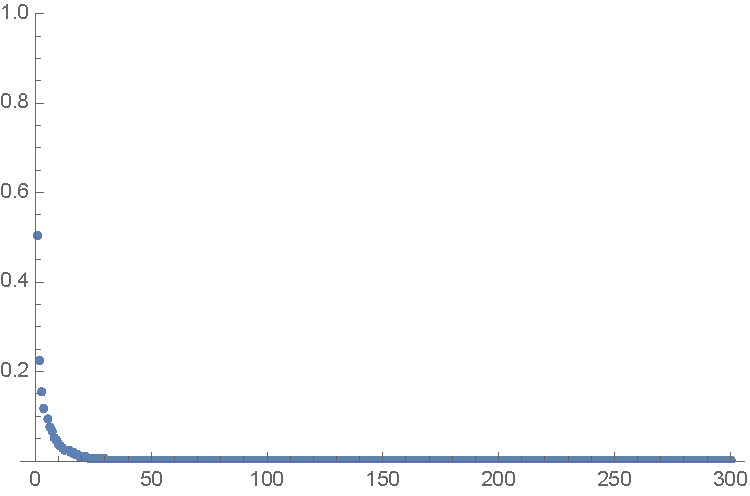
\includegraphics[width=0.4\textwidth]{a_09.pdf}
		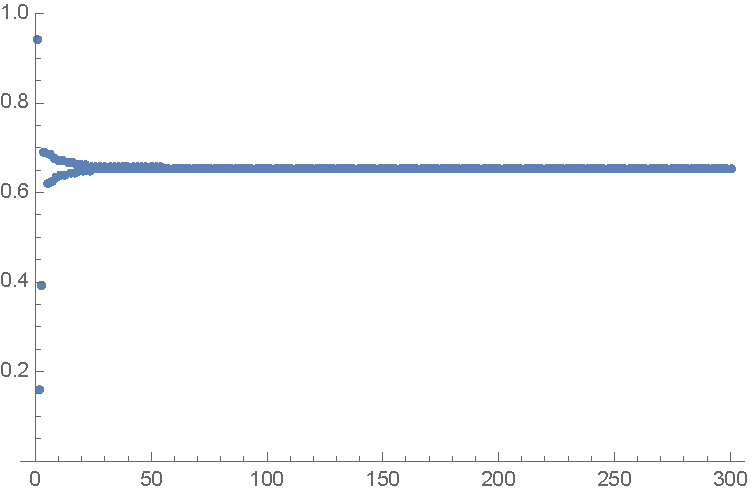
\includegraphics[width=0.4\textwidth]{a_29.pdf}
		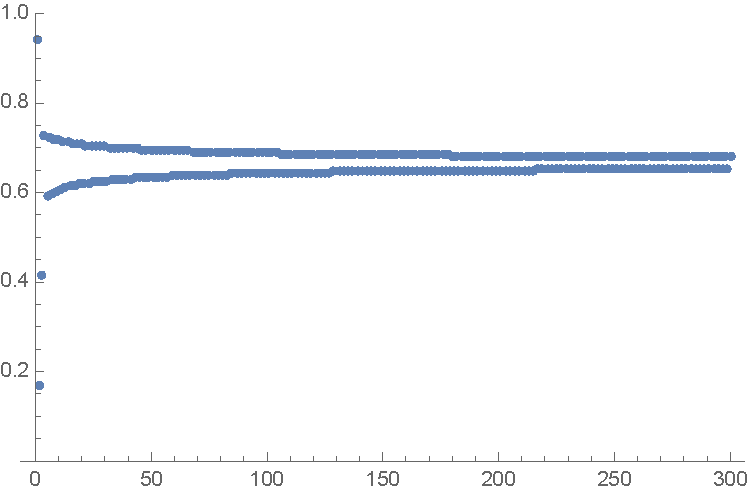
\includegraphics[width=0.4\textwidth]{a_30.pdf}
		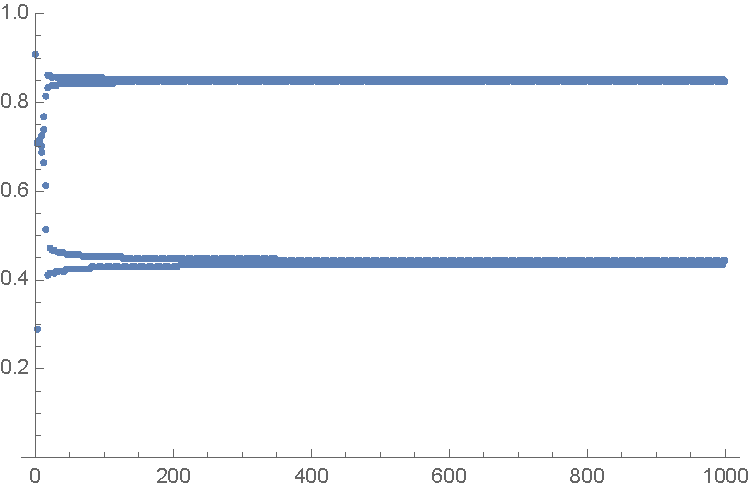
\includegraphics[width=0.4\textwidth]{a_3449.pdf}
		\caption{logistic map. Upper, left a=0.99, right a=2.9. Lower, left a=3.0, right a=3.4494.}
	\end{center}
\end{figure}

\section{Problem 5 to 7}
Find out bifurcation point for $2^m$-circle.  

\subsection{Theory}
\begin{figure}[h!]
	\begin{center}
		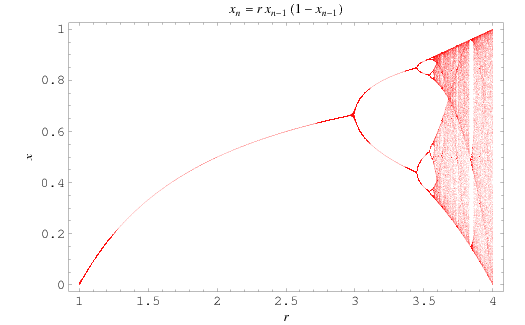
\includegraphics[width=0.8\textwidth]{logistic_map.png}
		\caption{bifurcation diagram of the logistic map. Pic. from Mahtworld}
		\label{fig1}
	\end{center}
\end{figure}
From experiment above, we know that when r goes to certain point, x iterate to 2 number. By introducing self-iterated function $x=f^m(x)=f(f(f(......(x))))$ we are able to find out analytical solution for $2^m$-order polynomial. In the other hand, we can use numerical approach to find the solution. By testing the multiplier
\begin{equation}
	\lambda=|\frac{x}{dx}f^m(x)|=\Pi^m_{n=0}f'(f^m(x))f'(f^{m-1}(x))...f'(x)<1
\end{equation} 
determined stability of $x$ given certain $a$. More, let $\lambda\rightarrow-1$ we can find the bifurcation point accurately.

\subsection{Algorithm}
Giving $m$, random initial value $x_0$ and starting $a$, $logistic$ returns $x_n (n=2000)$ of $2^m$-order iterated function. Use $x_n$ as initial guess plug into $Newton's method$
\begin{equation}
	x_{n+1}=x_n-\frac{f^m(x)-x}{f'^m(x)-1}
\end{equation}
stop at $x_{n+1}-x_n<10^-13$.

Multiplier calculated by equation demonstrated in (15). If $\lambda>-1$ then increasing a little step in parameter $a$, keep going on finding next $\lambda$ and determined its stability. Once $\lambda<-1$, I adjust step size to find more digit. Repeat it on the next period, which $m=m+1$

More, I test automatically survey of a by bisection method. Giving a interval $[a_0,a_1]$, if $\lambda>-1$, then make the right end to bisect point keep search $a$ to limit of computer digit.

\subsection{Sample output}
\subsubsection{2-perid bifurcation}
\begin{table}[t!]
	\begin{center}
		\begin{tabular}{c|c}
			\hline
			Parameters & \\ 
			\hline
			Logistic step & $1000$ \\
			Newton's accuracy& $10^{-12}$\\
			Total accuracy&$\epsilon<10^{-13}$\\
			\hline
		\end{tabular}
	\end{center}
	\caption{key parameters of algorithm}
\end{table}
Table 2. shows the key parameter of algorithm. Bisection method are applied to find optimized bracket. The procedure do not take too much steps to find the root on the limit of computer digits. Figure 2 shows the program output. 47 steps are taken and make the result as close as possible to analytical answer 3.0.

\begin{figure}[t!]
	\begin{center}
		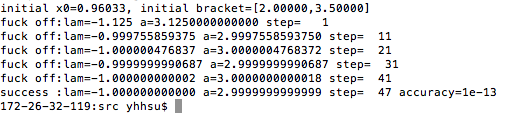
\includegraphics[width=0.8\textwidth]{sample_0.png}
		\caption{Numerical approach to 2-period-bifurcation point}
		\label{fig2}
	\end{center}
\end{figure}


\subsubsection{4-period bifurcation}
The approximation is great without changing the key parameters. The accuracy is exactly reach to computer's limit.  That is, $\epsilon=|a_{exp}-(1+\sqrt{6})|<10^{-13}$. Compare to 2-period, 4-period only take 2 more step converging to this precession.


\begin{figure}[h!]
	\begin{center}
		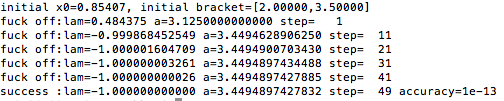
\includegraphics[width=0.8\textwidth]{sample_1.png}
		\caption{Numerical approach to 4-period-bifurcation point}
		\label{fig2}
	\end{center}
\end{figure}

\subsubsection{8-period bifurcation}
Here comes challenge. For some reason the program did not converge to $\lambda=-1$. Sometime Newton's method is fail to find the approximate root. I let the program change initial value when Newton's fail, and raising the iteration of logistic map in order to plug in better initial guess for root-finding. It turns out bisection always going out of the expected range and fail to converge. Although I give a very small initial bracket, $\lambda$ can not returns within $10^{-4}$ accuracy. Table 3 is key parameter in this exercise. 

In addition, I try to use step-in algorithm instead of bisection. It seems that my $\lambda$ is not smooth and continuous around fixed point. Figure 5 shows an example of step-in result. $\lambda$'s behavior is very sensitive to initial value. It make difficulties to get a consistent result of bifurcation point.

In the further period, the program behave like this and I am not able to find any point. Therefore, I am fail to show Feigenbaum constant and $r_{\infty}$.

\begin{figure}[h!]
	\begin{center}
		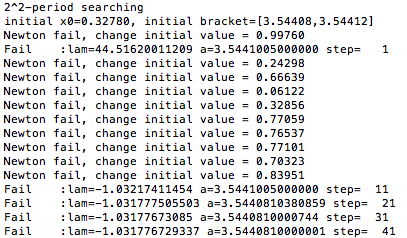
\includegraphics[width=0.8\textwidth]{sample_2_2.png}
		\caption{Numerical approach to 8-period-bifurcation point}
		\label{fig2}
	\end{center}
\end{figure}



\begin{table}[h]
	\begin{center}
		\begin{tabular}{c|c}
			\hline
			Parameters & \\ 
			\hline
			Logistic step & $10000$ \\
			Newton's accuracy& $10^{-12}$\\
			Total accuracy&$\epsilon<10^{-4}$\\
			\hline
		\end{tabular}
	\end{center}
	\caption{key parameters of algorithm}
\end{table}

\subsubsection{f(x)=Sin(pi*X)}
Simply change the definition of function and its derivative. I find the first four period bifurcation easily.
\begin{table}[h]
	\begin{center}
		\begin{tabular}{c|c}
			\hline
			period & bifurcation point a\\ 
			\hline
			2 & $0.7199616841972$ \\
			4 & $0.8332663532346$\\
			8 & $0.8591690091416$\\
			16& $0.8640801075000$*\\
			\hline
		\end{tabular}
	\end{center}
	\caption{Numerical approach to recursion sin function. First three are searching by bisection method, $\epsilon<10^{-10}$. *Last one is using step-in method, accuracy$\epsilon<10^{-5}$, although steps are much smaller than that.}
\end{table}
Calculating $Feigenbaum$ constant, I get
\begin{equation}
	\delta=\frac{0.8332663532356-0.719961841972}{0.8591690091416-0.8332663532346}=4.37
\end{equation}



\end{document}


\begin{table}[h!]
	\begin{tabular}{c|lr}
		\hline
		A & $Table$ & Is\\ 
		Messy & To & Write\\
		\hline
	\end{tabular}
\end{table}


\begin{figure}[b!]
	\begin{center}
		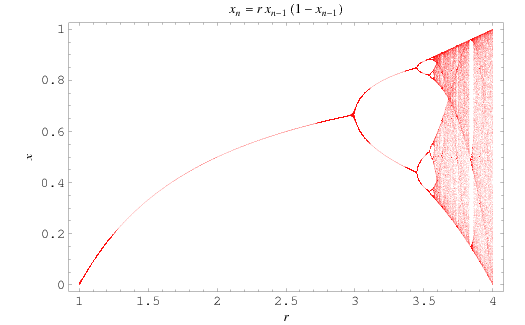
\includegraphics[width=0.8\textwidth]{logistic_map.png}
		\caption{bifurcation diagram of the logistic map. Pic. from Mahtworld}
		\label{fig1}
	\end{center}
\end{figure}
